\section{Rivers \& Streams}

In this section will be reviewed the various techniques that are used to place rivers and streams on a terrain. We will split the review material into the following categories, each with a dedicated section: \textit{Classification-based}, \textit{Simulation-based}, \textit{Heuristic-based} and \textit{Explicit}.\\ 
\textit{Classification-based} methods use pre-classified data based on real-world analysis to determine the most suited water network given a set of user-defined or terrain-defined constraints.\\
\textit{Simulation-based} techniques attempt to simulate natural phenomena such as gravity to determine the water networks on a given terrain.\\
\textit{Heuristic-based} techniques use algorithms based on real-world observation in an attempt to produce a plausible river network on the terrain. \\
\textit{Explicit} techniques require the user to specify in great detail the path the river should follow on the terrain.\\

The various techniques will be critiqued based on: the realism of the generated river networks, their computational cost and the level of automation they provide.

\subsection{Classification-based}

Classification-based methods use real-world analysis of river networks to determine, based on terrain parameters (slope, soil type, flow intensity, etc.), the types of rivers best suited (stream, cascade, rapid, etc.) to given landscapes.\\

Emilien et al \cite{Emilien2014} use classification-based techniques in their research focused on the lesser explored area of procedurally generated waterfall scenes. They model waterfalls as three separate segments: \textit{running water}, \textit{free-fall} and \textit{pool}. \textit{Running water} segments are parts of the water network in continuous contact with the terrain. \textit{Free-fall} segments are parts which break terrain contact (i.e. waterfall). Lastly, \textit{pool} segments represent the water-basin formed where free-fall segments meet the terrain. \\
Given a terrain, the user models running water and pool segments by defining control points and free-fall segments by defining a parabola. The control points for the running water and pool segments are not constrained to being in contact with the terrain as the terrain will adapt accordingly. The only constraint is that the path must continuously flow downhill. Based on this input, the system calculates plausible water flow intensities which, if required, can be overridden by the user for finer control.\\
The slope and water flow intensity requirements are then used as input to the waterfall classification (figure \ref{Waterfall classifications}) in order to determine realistic waterfall scenes to generate.\\

\begin{figure}[h]
  \centering
	\label{Waterfall classifications}
	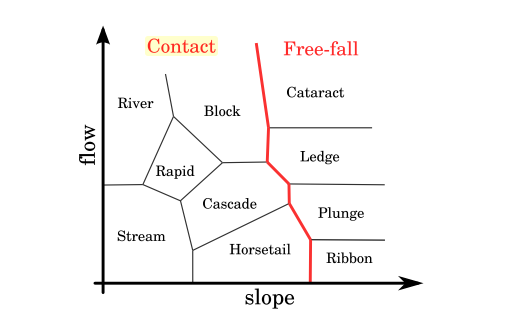
\includegraphics[]{waterfall_classification.png}
	\caption{Waterfall classifications \cite{Emilien2014}}
\end{figure}

By automatically generating plausible waterfall scenes based on trajectory input from the user, the technique strikes a good balance between automation and user control. A consequence of this, however, is that the resulting realism is heavily user-dependent. \\ 
In terms of computational complexity, the work by Emilien et al \cite{Emilien2014} is able to produce complex waterfall scenes in near real-time.

\subsection{Simulation-based}

Simulation-based techniques attempt to reproduce real-world phenomena to generate realistic river networks on given terrains. These simulations vary greatly in the level of detail they attempt to reproduce and can be split into the following sub-categories, each with a dedicated section below: \textit{Gravitation-simulation} \textit{Erosion-simulation} and \textit{Rainfall simulation} \\

\subsubsection{Gravity-simulation} \label{ssec:gravitation}

Gravity simulating techniques attempt to determine the path water will take on a terrain by algorithmically replicating the effects of gravity. \\

In order to generate plausible rivers, Belhadg et Audibert \cite{Belhadj2005} simulate the effect gravity has on water particles placed on the peaks of pre-generated ridges. To create the ridges, particle pairs are first placed at random locations on the terrain. These particle pairs are then randomly assigned a horizontal axis from which they iteratively distance themselves in opposite directions. At each iteration a new vertex is placed and its height decreased from the previous vertex based on a Gaussian distribution. To create the river networks, river particles are placed on the top of these generated ridges and a physical simulation which takes into consideration particle velocity, particle mass and surface friction is used to model the motion of these particles on the terrain. The path followed by these particles is tracked and, when two paths intersect, their particle velocity and mass are combined. When all particles have stopped moving the simulation is deemed balanced and all particle paths which do not lead to terrain extremities discarded. The remaining particle paths are kept and form the core river network. \\

Similarly, in the work by Soon Tee \cite{Teoh2008}, water is placed at specific locations on the terrain either by the user or whilst simulating rainfall. To determine the course the placed water takes on the terrain, water is iteratively evacuated into the surrounding cell with lowest elevation. This continues until a local minima or terrain extremities is reached.\\

In their work on modelling the effects of hydraulic erosion, Št'Ava et al. \cite{StAva2008} determine the course user-placed water takes on the terrain using a hydrostatic pipe-model simulation. In order to do so, the terrain is split into equal-sized (configurable) columns and the simulation iteratively evacuates water from source to surrounding destination columns based on column elevations, fluid density and gravitational acceleration. \\

These techniques can produce very plausible results but have the downside of being dependent on the base terrain as their height-field must cater for river networks in the first place. This is not the case, however, for the work by Št'Ava et al. \cite{StAva2008} fow which the gravitation simulation is used as a feedback loop to model terrain erosion. The performance of these methods depend heavily on the level of detail of the underlying water flow simulation. Št'Ava et al. \cite{StAva2008} succeed in generating the water flow in real-time by optimizing their algorithms to use the heavily parallel architecture of GPUs.

\subsubsection{Erosion-simulation}

Erosion-based simulations attempt to produce realistic terrains by modelling the effects of erosion. Erosion results from exogenic processes (water flow, wind, temperature) and is characterised by the removal of soil and rock from one location on earth's surface to be redeposited on another. Earth's landscape is a direct consequence of erosion and reproducing this phenomena accurately is core to procedurally generating accurate landscapes. Both Kelly et al. \cite{Kelley1988} and Št'Ava et al. \cite{StAva2008} attempt to produce plausible terrains by modelling these effects.\\

In the work by Kelley et al. \cite{Kelley1988}, the user specifies, on a horizontal plane, the terrain outline along with the main trunk stream. The terrain outline is used to configure the terrain extremities once ported to a three-dimensional space. The main trunk stream specifies the path which the highest order water stream should follow on the resulting terrain. Given this terrain outline and the position of the initial main trunk stream, the system iteratively increments the number of nodes which form the main trunk in order to add streams to the network. The number of new nodes added depends on the drainage area (surface area that a stream needs to channel) and the soil type as more resistant soil materials (e.g. stone) will be less influenced by water erosion than weaker ones (e.g. clay). \\

Št'Ava et al. \cite{StAva2008} are able to simulate the effects of hydraulic erosion on a terrain in real-time by using the massively parallel architectures of GPUs. Virtual pipettes are used by the user to drop water at required locations on the terrain and a gravitation simulation mentioned previously (\ref{gravitation-based}) is used to determine the initial water course on the terrain. Whilst the water is being routed through the terrain, the effects of \textit{force-based} and \textit{dissolution-based} erosion are simulated. \textit{Force-based} erosion is a direct consequence of the the force of the water on the terrain surface (figure \ref{force-based erosion}). Dissolution-based erosion is a consequence of the water mass on the terrain surface under the water and is most often characterised by a smoothing effect (figure \ref{dissolution_based_erosion-based erosion}).\\

\begin{figure}[h]
  \centering
	\label{dissolution_based_erosion-based erosion}
	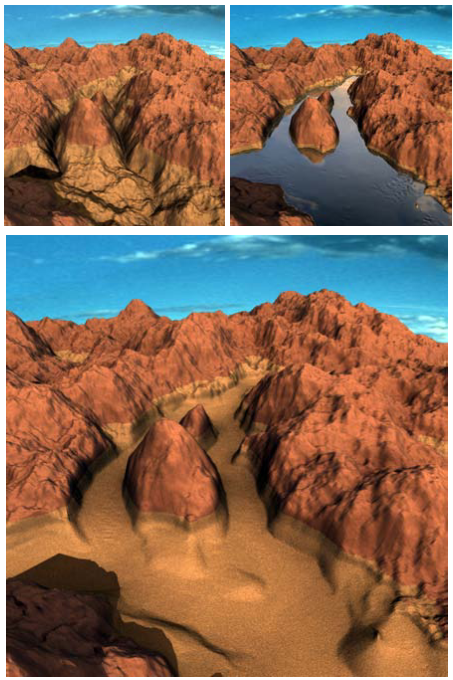
\includegraphics[scale=0.5]{dissolution_based_erosion.png}
	\caption{Simulation of dissolution-based erosion erosion caused by water movement\cite{StAva2008}}
\end{figure}

\begin{figure}[h]
  \centering
	\label{force-based erosion}
	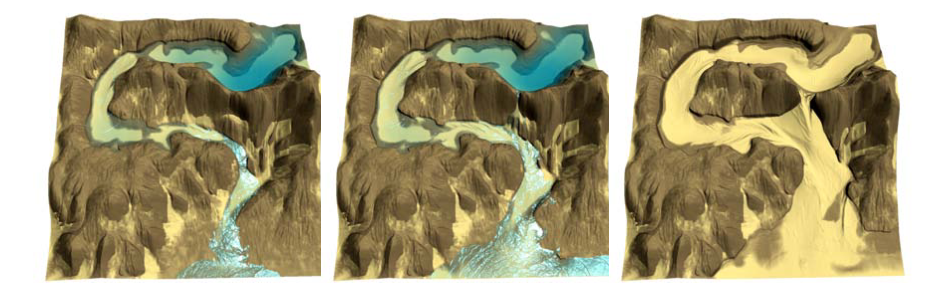
\includegraphics[width=\textwidth]{force_based_erosion.png}
	\caption{Simulation of the effect of force-based erosion caused by running water \cite{StAva2008}}
\end{figure}

Whether modelling erosion indirectly like in the work by Kelley et al. \cite{Kelley1988} which builds the terrain around models of erosion or directly like the work by Št'Ava et al. \cite{StAva2008} which simulates the effect of erosion in real-time, both succeed in producing plausible terrains with integrated river networks. Fine-control over the resulting terrain, however, is limited in the work by Kelley et al. \cite{Kelley1988} due to extensive automation. This is overcome in the work by \cite{StAva2008} et al. by permitting the user to both place water using a virtual pipette and remodel the terrain relief. In terms of computational cost, Št'Ava et al. \cite{StAva2008} are able to reproduce the effects of erosion in real-time.  

\subsubsection{Rainfall simulations}

In order to determine where on the terrain rivers will appear, work by Soon Tee \cite{Teoh2008} performs a rainfall simulation to determine both the location and quantity of water at different points on the terrain followed by a gravitation simulation (mentioned above) to determine the course of the water on the terrain. The rainfall simulation requires the user to specify wind direction and maximum rainfall. Then, starting from the source of the wind, the system simulates clouds moving in the direction of the wind with a configured velocity. When contact is made with points on the terrain, water is dropped on the corresponding cell. The amount of water dropped increases with altitude and zeroes out when all available rainfall is depleted. \\

Simulating rainfall in order to determine where water will fall on the terrain and therefore where river networks will form is an original approach and one that successfully generates visually plausible terrains. Requiring only wind direction, wind velocity and maximum rainfall from the user, the system provides a good level of automation. Determining the influence these inputs have on the resulting scene could be unintuitive, however, and require a "trial-and-error" approach. Their algorithm creates the  terrain along with the river networks in O(n) time, n representing the number of cells on the terrain.

\subsection{Heuristic-based}

Heuristic approaches attempt to build river and stream networks on terrains by algorithmically reproducing key characteristics based on real-world observations. \\

Derzapf et al. \cite{Derzapf2011} use such methods in their work based on procedurally generating virtual planets in real-time. To do so, only a very basic mesh-representation of the terrain is generated at first and detailed content is generated on demand as the user navigates through the virtual world. This method of adaptive rendering permits memory usage to me manageable whilst not compromising on realism. To ensure updates are performed in real-time, their algorithms are designed to make use of the massively parallel architecture of GPUs. \\
To initialise the base representation of the planets, the system first creates the base mesh with all vertices representing the sea. The system then randomly assigns a certain number of these vertices to act as seed continent vertices to spread until a user-configured land-to-water ratio is reached.
To place rivers, similarly to the work by \cite{Genevaux2013} et al., they first locate continental points which are on coastal edges to act as river mouths. When such a vertices are found, adjacent continental vertices are iteratively selected pseudo-randomly and connected in order to form the river network. \\
To assign ground altitudes to connected river vertices the system employs the following formula, starting from the river mouth:

\begin{center}
$a_{v} = a_{u} + e_{a}l_{e}\xi , e_{a} = \frac{a_{maxriver}}{l_{r}} $ \\
\end{center}

Where:
\begin{itemize}
\item $a_{v}$ is the ground altitude of the current vertex.
\item $a_{u}$ is the ground altitude of the previously processed vertex (or zero if \textit{v} is the first vertex).
\item $e_{a}$ is the average ground elevation.
\item $l_{e}$ is the length of the current vertex.
\item $\xi \in [0,1[$ is a uniformly distributed pseudo-random number.
\item $a_{maxriver}$ is the user-configured maximum river altitude.
\item $l_{r}$ is the current river length.
\end{itemize}

When the ground altitudes have been assigned, the following formula is used iteratively on each river vertex to assign water altitudes:

\begin{center}
$w_{v} = a_{v} + e_{w}l_{e}, e_{w} = \frac{\epsilon_{river}}{l_{cr}} $
\end{center}

Where:
\begin{itemize}
\item $w_{v}$ is the water altitude of the current vertex.
\item $a_{v}$ is the ground altitude of the current vertex.
\item $e_{w}$ is the average water elevation.
\item $l_{e}$ is the length of the current vertex.
\item $\epsilon_{river}$ is the user-configured maximum river depth.
\item $l_{cr}$ is the distance from the current vertex to the river spring.
\end{itemize}

All randomness in these algorithms depend on a configured seed value enabling the virtual world to be easily reproducible.  \\

\subsubsection{FRACTALS}

Another way to reproduce river streams heuristically is by employing fractal-based algorithms. Such methods use recursive splitting and string rewriting to determine plausible river networks. 

In their work, Pmsinkiewicz et al. use a fractal-based technique based on midpoint-displacement to procedurally generate plausible rivers on a terrain. Midpoint-displacement is most commonly used for procedurally generating realistic terrain height-maps and works follows follows: Given a starting triangle representing a terrain \textit{A}, midpoint-displacement iteratively subdivides \textit{A} it into four smaller triangles. Each time new triangle vertices are created they are displaced vertically by a random offset. This process is repeated until a given recursion limit is reached. See figure \ref{Midpoint displacement} for an example of a single iteration of the process.

\begin{figure}[h]
  \centering
	\label{Midpoint displacement}
	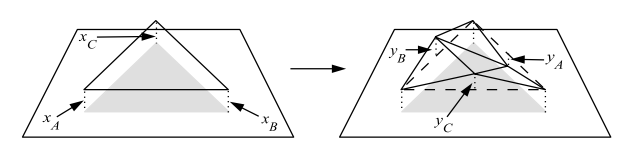
\includegraphics[width=\textwidth]{midpoint_displacement.png}
	\caption{A single iteration of midpoint displacement for the creation of mountains \cite{Prusinkiewicz1993}. New vertices $y_{A}$, $y_{B}$ and $y_{C}$ are created and shifted vertically by a random offset}
\end{figure}

To adapt this method to the generation of rivers on the terrain, rather than vertically displace newly formed triangle vertices, there edges are labelled as \textit{entry}, \textit{exit} or \textit{neutral} (figure \ref{Single production of midpoint displacement adapted to river generation. Given the initial triangle, four valid split scenarios.}). An \textit{entry edge} defines the point of entry for the river into the triangle, an \textit{exit edge} the point of exit and a \textit{neutral edge} prevents the river from passing through. \\

When a production step is applied and a triangle split, the following constraints must be applied:
\begin{itemize}
\item An entry edge must split into an entry and a neutral edge.
\item An exit edge must split into an exit edge and a neutral edge.
\item A neutral edge must split into two neutral edges.
\item The newly formed edge-pairs within the triangle must either be "entry/exit" or "neutral/neutral".
\end{itemize}

\begin{figure}[h]
  \centering
	\label{Single production of midpoint displacement adapted to river generation. Given the initial triangle, four valid split scenarios. }
	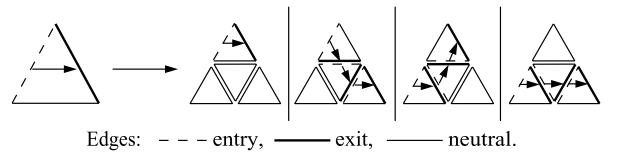
\includegraphics[width=\textwidth]{midpoint_displacement_for_rivers_1.png}
	\caption{Single production of midpoint displacement adapted to river generation \cite{Prusinkiewicz1993}. Given the initial triangle, four valid split scenarios.}
\end{figure}

One difficulty with this technique is to ensure two adjacent triangles are coherent once they split. That is, that the exit edge of one coincides with the entry edge of the other. To solve this, the location of edge vertices are used as the key to a random number generating hash table which, based on its output number, determines which segment will be crossed by the river.  \\

In their work, Génevaux et al. \cite{Genevaux2013} use fractal-based string rewriting to produce the river networks on the terrain. Once initial nodes have been heuristically selected to act as the river mouth, rewriting grammar is used to perform river node expansion. Configured values of $\rho_{a}, \rho_{s} and \rho_{c}$ influence the probability of selecting productions favouring asymmetric branching, symmetric branching and continuation without branching, respectively. The position for the new node is then selected based on the following constraints:
\begin{itemize}
\item It should be at a minimum distance from existing nodes and edges.
\item The new node should be at a greater distance from the terrain contour.
\item The new node should be compatible with the elevation constraints of existing nodes.
\end{itemize}
If a position satisfying these constraints is found, a new node is added at the given position and the process is repeated.\\

\subsection{Explicit}

Explicit techniques use explicit input from the user to determine locations and properties of the river networks to generate.\\

Flood-filling is such a technique and is used in the work by Soon Tee \cite{Teoh2008} to permit users to place water reserves (e.g. sea, lakes, etc.) by clicking a single point on the terrain. This point which will act as the seed point for the water surface and will propagate iteratively to surrounding points at lower heights until all such points have been depleted. \\

Smelik et al. also use explicit techniques to create an interactive system permitting users to model a complete virtual world with content ranging from rural features (mountains, rivers, etc.) to man-made ones (buildings, road networks). When modelling the virtual world, interactions are split into two modes: \textbf{Landscape} and \textbf{Feature}. \textit{Landscape mode} permits the designer to paint ecotopes onto the terrain using traditional image editing tools. These ecotopes are predefined by the user and encompass both elevation and soil material information. In \textit{feature mode}, the user is able to place terrain content, including rivers. To do so, similarly to the interface provided by Emilien et al. \cite{Emilien2014}, the user sketches vector lines outlining the core path of the river and, based on this, a suitable course is plotted through the landscape. Other terrain features to which the river takes precedence adapt accordingly. For example, if the river is plotted to pass through a forest, trees on the rived bed and bank will be removed automatically. \\

Rather than placing vector-lines, the work by Soon Tee \cite{Teoh2008} and Št'Ava et al. \cite{StAva2008} permits users to click single points on the terrain which will act as the water source. The system then automatically generates a plausible path for the water down slope of the terrain.